\chapter{Introduction} \label{ch:Introduction}

%Here comes the introduction. Explain why the topic of your thesis is important and what is the goal of the thesis. If you need, use references like this \cite{higham2020handbook}. If you want to use acronyms, define a \textit{newacronym} in the file "sybol\_directory.tex" and use it like this: \gls{lti}. The next time you use the acronym \gls{lti} is appears authomatically in short form.  
%
%You can also include images like this.
%\begin{figure}[ht!]
%    \centering
%    
\includegraphics[width=\textwidth]{03_images/meme.png}
%    \caption{Graphical representation of the research process.}
%    \label{fig:Introduction:meme}
%\end{figure}
%
%
%A meme can be seen in Figure~\ref*{fig:Introduction:meme}. This demonstrates that 
%\begin{equation} \label{eq:Introduction:realisation}
%	1 \le 2 \ \text{or} \ 1 \ge 2.
%\end{equation}
%In addition to \eqref{eq:Introduction:realisation}, it could be postulated that $1 \ne 2$. Further discussions are considered in the following sections and subsections.

\newtheorem{definition}{Definition}
\section{Background and Motivation} \label{sec:Introduction:Background}

Robots are used extensively in manufacturing, not only in the automotive industry but also in the production of the space shuttle, the development of military equipment and high-speed railways, and the production of commodities. Due to the rapid development of robotics, not only is the price gap between products becoming smaller and smaller compared to traditional industrial equipment, but also the degree of personalization of products so that industrial robots can be used to replace traditional equipment in the manufacture of some complex products, which can vastly improve economic efficiency and save energy \cite{EEUIR}.

The use of robots in factories can solve many safety problems. Potential safety problems for personal reasons, such as unfamiliarity with work processes, negligence, or fatigue, can be avoided.

As robotics continues to develop and advance, an individual robot can no longer perform complex and tedious tasks independently to meet the work targets in production practice, and there is an urgent need to research new directions to meet practical needs. Multiple robots working simultaneously can increase efficiency and enhance the synergy of work task indicators. Systems made up of multiple robots have certain advantages over an individual robot \cite{PFRCD}.

	(1) High adaptability to the environment: Compared to individual robots, multi-robot systems show greater flexibility and adaptability to work tasks, with better distribution in function and space than individual robots.

	(2) Strong load-bearing capacity: A multi-robot system is a group, with each robot working individually while coordinating with the others, resulting in much shorter working times, effectively increasing productivity and a more substantial work-bearing capacity.
	
	(3) High robustness. In multi-robot systems, task completion requires the involvement of each robot rather than relying exclusively on one robot, thus providing high fault tolerance and robustness.

Industrial robots have evolved from traditional handling, assembly, and welding tasks to a wide range of production applications. The use of robots in manufacturing processes can lead to high flexibility and low costs. However, the performance of robots is hardly comparable to that of machine tools. Stiffness is considered to be a significant weakness in robotic machining applications \cite{MIIR}.

Using two coupled robots in manufacturing provides higher stiffness than one robot. To reduce defects in robotic machining, physically coupled multi-robot systems are used. Physically coupled robots perform coordinated actions through force interactions. The end-effectors or flanges of several robots can be connected utilizing a rigid coupler. Various machining tasks, such as drilling and milling, can be implemented on the coupler by employing ratchets attached to the coupler. Most stiffness problems in robot-driven machining research have been on a single robot \cite{WPOIR} \cite{POMIR}  \cite{SOPO}, and there is a need to extend these studies to multi-robot systems. 

In order to increase the stiffness of the coupled robot, an optimization method is used to find the optimal pose of coupled robots, position, and angle of the workpiece.



%\subsection{Contribution of my thesis}
%
%text text text text text text text text text text text text text text text text text text text text text text text text text text text text text text text text text text text text text text text 

\section{Problem Definition} \label{sec:Introduction:Problem Definition}

\begin{definition}[Stiffness]
	Stiffness is the extent to which an object resists deformation in response to an applied force.
\end{definition}

\begin{figure}[h!]
	\centering
	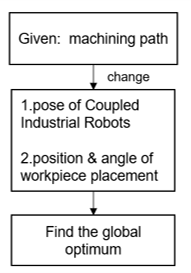
\includegraphics[width=\textwidth]{03_images/process.png}
	\caption{Graphical representation of the research process.}
	\label{fig:Introduction:meme}
\end{figure}





